\documentclass[a4paper, 11pt]{report}
\usepackage[utf8]{inputenc}
\usepackage{amsmath,tabto}
\usepackage[hidelinks]{hyperref}
\usepackage{titlesec}
\titleformat{\chapter}[display]
  {\normalfont\bfseries}{}{0pt}{\Huge}
\usepackage{graphicx}

\usepackage{glossaries}
\graphicspath{ {images/} }
\date{null}
\usepackage{fullpage} % changes the margin
\usepackage{setspace}
\usepackage{multirow}
\begin{document}
\begin{titlepage} % Suppresses displaying the page number on the title page and the subsequent page counts as page 1
	\newcommand{\HRule}{\rule{\linewidth}{0.5mm}} % Defines a new command for horizontal lines, change thickness here
	
	\center % Centre everything on the page
	
	%------------------------------------------------
	%	Headings
	%------------------------------------------------
	
	\textsc{\LARGE Concordia University}\\[1.5cm] % Main heading such as the name of your university/college
	

	%------------------------------------------------
	%	Title
	%------------------------------------------------
	
	\HRule\\[0.4cm]
	
	{\huge\bfseries  SOEN 6481 - Software Design  Methodologies}\\[0.4cm] % Title of your document
	
	\HRule\\[1.5cm]
	\textsc{\Large Deliverable 1}\\[0.5cm] % Major heading such as course name
	\textsc{\Large Requirement Analysis for Ticket Vending Machine}\\[0.5cm]
	%------------------------------------------------
	%	Author(s)
	%------------------------------------------------
	
% 	\begin{minipage}{0.4\textwidth}
% 		\begin{flushleft}
			
% 			\end{flushleft}
% 	\end{minipage}
	~
% 	\begin{minipage}{0.4\textwidth}
% 		\begin{flushright}
			\large
			\textit{Supervisor}\\
			Prof. Pankaj Kamthan\\[0.5cm] % Supervisor's name
% 		\end{flushright}
% 	\end{minipage}
    \vfill
    \large
            \textbf{Team K}\\
			\textit{Authors}\\
		Devanshi Piyushkumar Patel - \textsc{40172139}\\
            Hetul Patel - \textsc{40225667}\\
            Jay Bharatbhai Patel - \textsc{40197003}\\
            Juhi Birju Patel - \textsc{40190446}\\
            Krishna Patel - \textsc {40206701}\\
            Mahavir Patel - \textsc {40198619}\\[0.75cm]
            
	
	% If you don't want a supervisor, uncomment the two lines below and comment the code above
	%{\large\textit{Author}}\\
	%John \textsc{Smith} % Your name
	
	%------------------------------------------------
	%	Date
	%------------------------------------------------
	
	\vfill\vfill\vfill\vfill% Position the date 3/4 down the remaining page
	\textbf{GitHub Address:} \url{https://github.com/mahavir0/iGo---SOEN-6461-SDM}

	%------------------------------------------------
	%	Logo
	%------------------------------------------------
	
 	\vfill\vfill
 	\includegraphics[scale=1.5]{download.png}\\[1cm] % Include a department/university logo - this will require the graphicx package
	 
	%----------------------------------------------------------------------------------------
	
	\vfill % Push the date up 1/4 of the remaining page
	
\end{titlepage}

%----------------------------------------------------------------------------------------


 
\tableofcontents
\chapter{Problem 1}
\section{Introduction}
In this document, the online ticket vending machine that is available in Montreal, Canada, will be examined and discussed. The project's goal is to produce a collection of related artifacts for the issue at hand as well as the domain of the software solution for a useable, secure, maintainable, and (environmentally) sustainable TVM. \\\\
The requirements and use cases are recorded in the pictorial representation with the help of problem domain, stakeholders and use case modelling and various other UML diagrams to understand different perspectives of the system.

\section{Description of iGo}
The term "TVM" refers for "Ticket Vending Machine," a self-service kiosk where customers may buy tickets for public transportation, including buses, trains, and subways. TVMs are intended to reduce the need for human interaction and speed up boarding time by making the ticket purchase procedure quick and simple for commuters. \\\\
After drawing inspiration from the present version of the TVM that STM has deployed notably in the metro system of Montreal, Canada, we chose to give alternatives for purchasing a ticket in numerous conceivable ways with our version of iGo. The various possible ways include single trip pass, one-day pass, two-day pass, weekly pass, and monthly pass. Customers may tap their card at any metro station to move effortlessly between different locations with the use of only one electronic fare card. \\\\
Moreover, users of iGo will have access to an online portal to reload their electronic cards and track all transactions from a single location. iGo will also make use of developing technology for making payments via secure channels utilising debit/credit cards.\\\\
With iGO, it is assumed that metro stations and buses have kiosks on which the application will be installed, to scan and validate the electronic tickets. Notwithstanding the fact that there is no provision in iGo for maintaining the existing physical TVMs available at metro stations in Montreal. 
\\\\
At the end of our project, we want to have created software that is useful and with capabilities similar to those of the Montreal metro TVM.  \\\\
iGo will provide a range of services related to purchasing and managing the transit tickets. Some of the services that will be provided include: 

\begin{itemize}
  \item \textbf{Ticket purchasing:} iGo will enable users to swiftly and conveniently tickets, minimising the need for human interaction and speeding up boarding time.
  \item \textbf{Ticket type selection:} Users can choose between single trip tickets, day passes, weekly or monthly passes, and other sorts of transit prices.
  \item \textbf{Payment processing:} iGo will accept cash, credit, or debit card payments, and even allow mobile payments like apple pay or phonepe.
  \item \textbf{Ticket printing:} iGo will provide tickets electronic tickets which the user can scan at the metro stations using the kiosks available there.
  \item \textbf{Multilingual support:} As Montreal is a French dominated city hence iGo will provide the support for two major languages namely English and French.
  \item \textbf{Account management:}iGo will allow its users to manage their transit accounts, by reloading or renewing passes, monitoring transaction history, and altering account information.
\end{itemize}
\leavevmode
\\
It should be noted here that implementing the payment gateways for purchasing the tickets is currently not within the scope for this project. However, a Payment option is added which can be extended for realization.
\\


\section{Future Scope}
Considering historical experience, we may anticipate that as Montreal's economy expands, additional stations will be built in the future years.
We will attempt to develop the TVM software so that it will be simple to update and add new needs while keeping these modifications in mind. 


\chapter{Problem 2}
\begin{figure}[h]
    \centering
    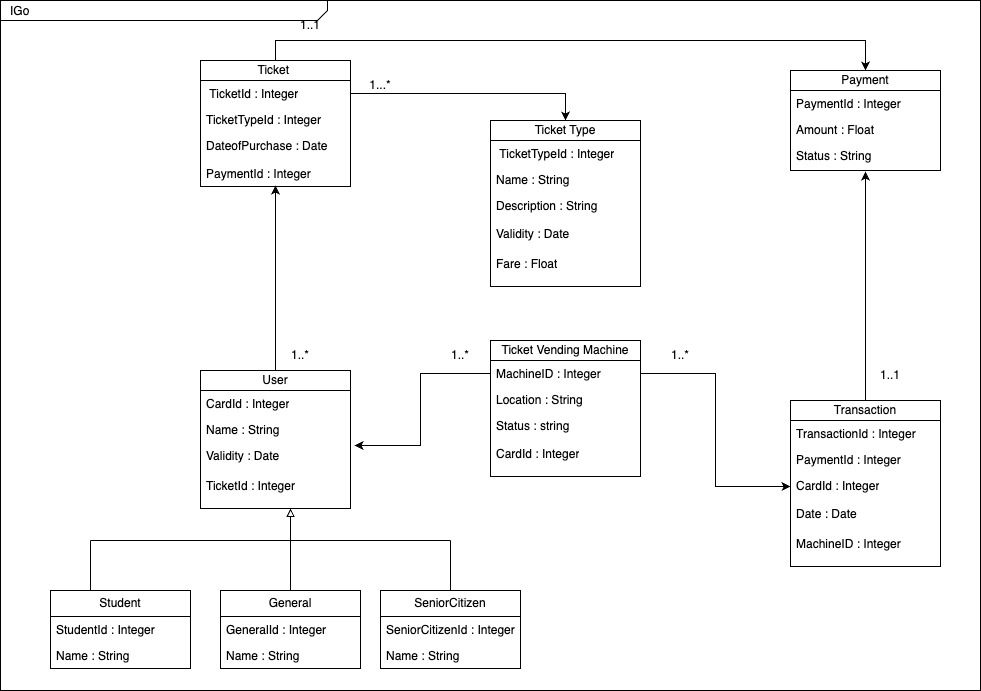
\includegraphics[scale=0.35]{Problem2_UML_iGo.jpg}
    \caption{UML Class diagram for iGo TVM}
    \label{fig:UML class diagram for iGo TVM}
\end{figure}


\section{Description about Classes}
The domain model consists of the following classes:

\begin{itemize}
  \item \textbf{Ticket: }
    This class represents a ticket that can be purchased from the TVM for a means of public transportation. It has the following attributes:
    \begin{itemize}
    \item validityPeriod: the duration for which the ticket is valid
     \item purchaseDate: the Date on which ticket was purchased
     \item payment: the details about the payment of this purchase
    \end{itemize}  
          
    \item \textbf{TicketType: }This class represents the types of tickets that can be purchased from the TVM. 
    It has the following attributes:
        \begin{itemize}
        \item name: the name of the ticket type
        \item description: a description of the ticket type
        \item validityPeriod: the duration for which the ticket is valid
        \item fare: the cost of the ticket
        \end{itemize}
     \end{itemize}   
     
  \item \textbf{Payment: } This class represents a payment made by the user to purchase a ticket from the TVM. It has the following attributes:
    \begin{itemize}
    \item amount: the amount of money paid by the user
    \item paymentMethod: the method used for payment (e.g. cash, credit card, mobile payment
    \item paymentStatus: the current status of the payment (e.g. success, fail) 
  
    
    \item \textbf{User: }  This class represents a user of the TVM system. It has the following attributes:
       \begin{itemize}
       \item  name: the name of the user
        \item email: the email address of the user
        \item password: the password of the user's account
        \item validity: the validity of the user's account
        \end{itemize}
        This class has three subclasses:
        \begin{itemize}
        \item Student
        \item General
        \item Senior Citizen
         \end{itemize}
          
     \end{itemize}

  \item \textbf{TVM: } This class represents the ticket vending machine itself. It has the following attributes:
\begin{itemize}
\item location: the physical location of the TVM
\item status: the current status of the TVM (e.g. operational, out of order)
\item serialNumber: the unique identifier for the TVM
 \end{itemize}

\item \textbf{ Transaction: } This class represents a transaction made by a user at the TVM to purchase a ticket. It has the following attributes:
\begin{itemize}
\item ticket: the ticket that was purchased
\item payment: the payment made by the user for the ticket
\item user: the user who made the transaction
\item date: the date and time the transaction was made
\item  Machine: the machine used to make the transaction
 \end{itemize}

\section{Description about Relationship among Classes}
\begin{itemize}
\item Ticket has a composition relationship with TicketType, as each Ticket is associated with a specific TicketType.
\item Transaction has a composition relationship with Ticket and Payment, as each transaction involves the purchase of a ticket and a payment made by the user.
\item Transaction has an association relationship with User, as each transaction is associated with a specific user.
\item Transaction has an association relationship with TVM, as each transaction is associated with the TVM that was used to make the transaction.
 \end{itemize}


\chapter{Problem 3}
\section{Mind Map}

The mind map for the ticket vending machine has several branches, each of them representing the different aspects of the given project. The main point for creating the mind map could be Ticket Vending Machine. \\
The given mind map includes mainly six branches security, Tasks, Payment Methods, User, Accessibility, and Usability. These branches could provide a summary of the report and their findings, as well as any recommendations for future improvements. \\
Overall, The given mind map for the ticket vending machine provides the scenario of various topics covered in this report. It would also help the reader to understand the structure and the flow of various tasks and make it easier for the presentation.\\


\begin{figure}[h]
    \centering
    \includegraphics[scale=0.35]{iGo-Mind_map.png}
    \caption{Mind Map for Interview of iGo TVM}
    \label{fig:Mind Map for Interview for iGo TVM}
\end{figure}

\chapter{Problem 4}
\section{Use Case Modeling}
\begin{figure}[h]
    \centering
    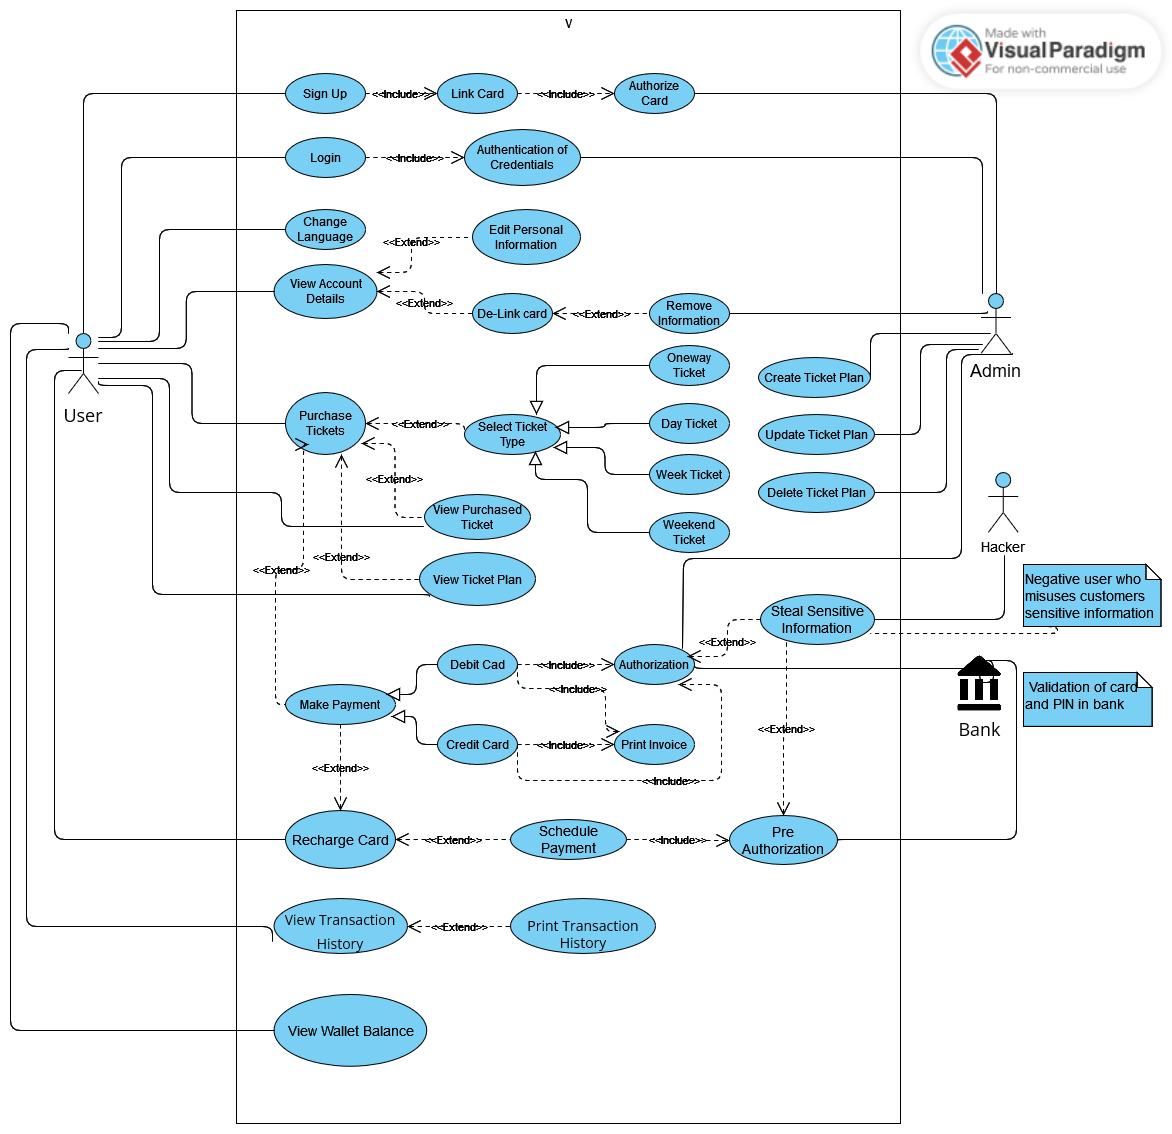
\includegraphics[scale=0.35]{Use_Case_Diagram.png}
    \caption{Use Case Model for iGo TVM}
    \label{fig:Use_Case_Diagram}
\end{figure}
\\\\

\noindent The iGo Ticket Vending Machine and the commuter or user are the key two actors in the use case model.
The user's use cases include logging in or signing up, choosing a language, purchasing tickets, topping off cards, paying for tickets and cards, and accessing account information, including transaction history and wallet balance.
Whereas iGo will handle the internal connection to the bank and the sorts of tickets that are shown.
In addition to these actors, there are two more: the Bank, which handles the authentication and verification of all credit card and debit card payment transactions, and the negative use case actor, the Hacker, who could attempt to breach the system, steal user data, and exploit it for their own advantage. 
\\\\
\renewcommand{\arraystretch}{1.5}
\begin{tabular}{ |l|p{11cm}| } 
\hline
 Name & Sign Up\\
 \hline
 ID  & UC1\\
\hline
Description & Customers want to Sign Up for TVM.\\
\hline
Actors & Customer and TVM System\\
\hline
Main Success Scenario   & \begin{tabular}{@{\labelitemi\hspace{\dimexpr\labelsep+0.5\tabcolsep}}p{0.9\linewidth}@{}}Customer needs to provide details like name, age, email address, password,date of birth etc.\\
Customers may have to provide valid documents if needed.\\ 
Customers have to submit the form.\\
Customers are asked to login in TVM.\\\end{tabular}  \\ 
\hline
Pre-Condition & Customers need to have some pre knowledge about how to use TVM.\\
\hline
Post-Condition & Customers need to login.\\
\hline
Exceptions/Alternatives & Customers failed to provide correct details.\\
\hline
\end{tabular}
\\\\
\\\\
\renewcommand{\arraystretch}{1.5}
\begin{tabular}{ |l|p{11cm}| } 
\hline
 Name & Login\\
 \hline
 ID  & UC2\\
\hline
Description & Customers want to login in the TVM System.\\
\hline
Actors & Customer and TVM System\\
\hline
Main Success Scenario   & \begin{tabular}{@{\labelitemi\hspace{\dimexpr\labelsep+0.5\tabcolsep}}p{0.9\linewidth}@{}}Customers have to know about login Credentials.\\ 
Customers are logged into the TVM System.\\ 
Customers can see the entire application.\\\end{tabular}  \\ 
\hline
Pre-Condition & Customers have to be aware of their credentials.\\
\hline
Post-Condition & Customers easily see all the details of the application.\\
\hline
Exceptions/Alternatives & \begin{tabular}{@{\labelitemi\hspace{\dimexpr\labelsep+0.5\tabcolsep}}p{0.9\linewidth}@{}}Customers have to check the credentials.\\
Customers need to register first if they do not already have an account.\\\end{tabular}  \\
\hline
\end{tabular}
\\\\
\\\\
\renewcommand{\arraystretch}{1.5}
\begin{tabular}{ |l|p{11cm}| } 
\hline
 Name & Change Language\\
 \hline
 ID  & UC3\\
\hline
Description & Users want to change the language.\\
\hline
Actors & Customer and TVM System\\
\hline
Main Success Scenario   & \begin{tabular}{@{\labelitemi\hspace{\dimexpr\labelsep+0.5\tabcolsep}}p{0.9\linewidth}@{}}Customers can alter the language between French and English\\\end{tabular}  \\ 
\hline
Pre-Condition & N/A\\
\hline
Post-Condition & They successfully change it.\\
\hline
Exceptions/Alternatives & Language is not available which they want.\\
\hline
\end{tabular}
\\\\
\\\\
\renewcommand{\arraystretch}{1.5}
\begin{tabular}{ |l|p{11cm}| } 
\hline
 Name & View Account Details\\
 \hline
 ID  & UC4\\
\hline
Description & Customers want to see the details related to their account.\\
\hline
Actors & Customer and TVM System\\
\hline
Main Success Scenario   & \begin{tabular}{@{\labelitemi\hspace{\dimexpr\labelsep+0.5\tabcolsep}}p{0.9\linewidth}@{}}Customers can see all the details which are a part of their personal profile.\\ 
Customers can also edit these details.\\ 
Customers can delink their registered card.\\
Customers can remove some details like saved payment methods.\\\end{tabular}  \\ 
\hline
Pre-Condition & They must know the credentials of the TVM System.\\
\hline
Post-Condition & It gives the option for users to edit or delete certain information.\\
\hline
Exceptions/Alternatives & Users have to provide some necessary additional information.\\
\hline
\end{tabular}
\\\\
\\\\
\renewcommand{\arraystretch}{1.5}
\begin{tabular}{ |l|p{11cm}| } 
\hline
 Name & Purchase Tickets\\
 \hline
 ID  & UC5\\
\hline
Description & Customers are able to  purchase tickets from various options available.\\
\hline
Actors & Customer and TVM System\\
\hline
Main Success Scenario   & \begin{tabular}{@{\labelitemi\hspace{\dimexpr\labelsep+0.5\tabcolsep}}p{0.9\linewidth}@{}}Customer can look at the different type of tickets available like one day pass,week pass, weekend pass and  one way trip pass.\\ 
Customers can view their purchased ticket.\\ 
Customers can also view the plan they purchased like monthly recharge, 3 month recharge or limited trip recharge.\\\end{tabular}  \\ 
\hline
Pre-Condition & They must login to the TVM system.\\
\hline
Post-Condition & It provides the details about the ticket plan or ticket purchased.\\
\hline
Exceptions/Alternatives & \begin{tabular}{@{\labelitemi\hspace{\dimexpr\labelsep+0.5\tabcolsep}}p{0.9\linewidth}@{}}Users have to login first to see plans.\\
Customer has not booked any tickets.\\\end{tabular}  \\
\hline
\end{tabular}
\\\\
\\\\
\renewcommand{\arraystretch}{1.5}
\begin{tabular}{ |l|p{11cm}| } 
\hline
 Name & Make Payment\\
 \hline
 ID  & UC6\\
\hline
Description & Customer makes the payment.\\
\hline
Actors & Customer,Bank and TVM System\\
\hline
Main Success Scenario   & \begin{tabular}{@{\labelitemi\hspace{\dimexpr\labelsep+0.5\tabcolsep}}p{0.9\linewidth}@{}}Customers get different options related to payment method like cash, credit card or debit card.\\ 
Customers need to select the method and proceed with the payment according to the given instructions. \\ 
 the payment is by card, Bank will provide verification and provide the authorization to make the payment.\\
Customer can also cancel the payment and go for change the plan.\\
After the payment is successful users get the option for printing their invoice.\\\end{tabular}  \\ 
\hline
Pre-Condition & Users must select the plan of Tickets.\\
\hline
Post-Condition & Users get the details of the bill and method of the payment.\\
\hline
Exceptions/Alternatives & \begin{tabular}{@{\labelitemi\hspace{\dimexpr\labelsep+0.5\tabcolsep}}p{0.9\linewidth}@{}}Users need to check the details of the card or pin which they provide to make payments.\\
Cancel the payment and want to go back?\\\end{tabular}  \\
\hline
\end{tabular}
\\\\
\\\\
\renewcommand{\arraystretch}{1.5}
\begin{tabular}{ |l|p{11cm}| } 
\hline
 Name & Recharge Card\\
 \hline
 ID  & UC7\\
\hline
Description & Users also recharged the card.\\
\hline
Actors & Customer,Bank and TVM System\\
\hline
Main Success Scenario   & \begin{tabular}{@{\labelitemi\hspace{\dimexpr\labelsep+0.5\tabcolsep}}p{0.9\linewidth}@{}}User needs to select the card recharge option namely one month unlimited, 3 month unlimited or limited trips recharge. \\
User needs to enter the details of their electronic card.\\ 
Users can proceed with the payment.\\\end{tabular}  \\ 
\hline
Pre-Condition & Users must insert the card.\\
\hline
Post-Condition & Customers have to confirm and have to proceed with payment.\\
\hline
Exceptions/Alternatives & \begin{tabular}{@{\labelitemi\hspace{\dimexpr\labelsep+0.5\tabcolsep}}p{0.9\linewidth}@{}}Please select from the above mentioned option only.\\
Cancel the payment.\\\end{tabular}  \\
\hline
\end{tabular}
\\\\
\\\\
\renewcommand{\arraystretch}{1.5}
\begin{tabular}{ |l|p{11cm}| } 
\hline
 Name & View Transaction History\\
 \hline
 ID  & UC8\\
\hline
Description & Customers also see all the transactions which they did till date.\\
\hline
Actors & Customer and TVM System\\
\hline
Main Success Scenario   & \begin{tabular}{@{\labelitemi\hspace{\dimexpr\labelsep+0.5\tabcolsep}}p{0.9\linewidth}@{}}Customers get the details like date and time of the transaction, method of payment etc of all the transactions successfully.\\Customers can also print the transaction history available.\\\end{tabular}  \\ 
\hline
Pre-Condition & Users have to log in with their credential\\
\hline
Post-Condition & They get all the history of transactions.\\
\hline
Exceptions/Alternatives & N/A\\
\hline
\end{tabular}
\\\\
\\\\
\renewcommand{\arraystretch}{1.5}
\begin{tabular}{ |l|p{11cm}| } 
\hline
 Name & View Wallet Balance\\
 \hline
 ID  & UC9\\
\hline
Description & Users can view their wallet balance.\\
\hline
Actors & Customer and TVM System\\
\hline
Main Success Scenario   & \begin{tabular}{@{\labelitemi\hspace{\dimexpr\labelsep+0.5\tabcolsep}}p{0.9\linewidth}@{}}They get the information about how much balance is available in their wallet.\\ 
Users also get an option to add more money in their wallet.\\\end{tabular}  \\ 
\hline
Pre-Condition & Users must be logged in to the TVM System.\\
\hline
Post-Condition & Users get the information in their account.\\
\hline
Exceptions/Alternatives & N/A\\
\hline
\end{tabular}
\\\\
\\\\
\renewcommand{\arraystretch}{1.5}
\begin{tabular}{ |l|p{11cm}| } 
\hline
 Name & Steal Sensitive Information\\
 \hline
 ID  & UC10\\
\hline
Description & Hackers use the TVM System unethically.\\
\hline
Actors & Hackers and TVM System\\
\hline
Main Success Scenario   & \begin{tabular}{@{\labelitemi\hspace{\dimexpr\labelsep+0.5\tabcolsep}}p{0.9\linewidth}@{}}Hackers used the TVM system improperly.\\
The user’s sensitive information is stolen by Hackers.\\
Hackers use this sensitive information for thrie personal gain.\\\end{tabular}  \\ 
\hline
Pre-Condition & The user inserted the card and entered the pin.\\
\hline
Post-Condition & The TVM System was hacked.\\
\hline
Exceptions/Alternatives & Perform illegal activity in your account.\\
\hline
\end{tabular}
\\\\
\\\\
\renewcommand{\arraystretch}{1.5}
\begin{tabular}{ |l|p{11cm}| } 
\hline
 Name & Create Ticket Plan\\
 \hline
 ID  & UC11\\
\hline
Description & Administrator wants to create the ticket plan.\\
\hline
Actors & Administrator and TVM System\\
\hline
Main Success Scenario   & \begin{tabular}{@{\labelitemi\hspace{\dimexpr\labelsep+0.5\tabcolsep}}p{0.9\linewidth}@{}}Administrator creates the new ticket plan.\\
Administrator can create a new ticket by adding all related information.\\\end{tabular}  \\ 
\hline
Pre-Condition & Administrator is logged in.\\
\hline
Post-Condition & New tickets are clearly visible in the Ticket plan screen.\\
\hline
Exceptions/Alternatives & N/A\\
\hline
\end{tabular}
\\\\
\\\\
\renewcommand{\arraystretch}{1.5}
\begin{tabular}{ |l|p{11cm}| } 
\hline
 Name & Update Ticket Plan\\
 \hline
 ID  & UC12\\
\hline
Description & Administrator wants to update an existing ticket plan.\\
\hline
Actors & Administrator and TVM System\\
\hline
Main Success Scenario   & \begin{tabular}{@{\labelitemi\hspace{\dimexpr\labelsep+0.5\tabcolsep}}p{0.9\linewidth}@{}}Administrator selects the tickets which they want to update.\\
Then modify it properly.\\
Administrator saves the changes.\\\end{tabular}  \\ 
\hline
Pre-Condition & Administrator is logged in.\\
\hline
Post-Condition & Update tickets are clearly visible in the Ticket plan screen.\\
\hline
Exceptions/Alternatives & N/A\\
\hline
\end{tabular}
\\\\
\\\\
\renewcommand{\arraystretch}{1.5}
\begin{tabular}{ |l|p{11cm}| } 
\hline
 Name & Delete Ticket Plan\\
 \hline
 ID  & UC13\\
\hline
Description & Administrator wants to delete the ticket plan.\\
\hline
Actors & Administrator and TVM System\\
\hline
Main Success Scenario   & \begin{tabular}{@{\labelitemi\hspace{\dimexpr\labelsep+0.5\tabcolsep}}p{0.9\linewidth}@{}}Administrator selects the ticket plan which they want to delete.\\
Administrator deletes it.\\\end{tabular}  \\ 
\hline
Pre-Condition & Administrator is logged in.\\
\hline
Post-Condition & Delete tickets are not visible in the Ticket plan screen.\\
\hline
Exceptions/Alternatives & There are no tickets selected to delete.\\
\hline
\end{tabular}




\chapter{Problem 5}
\section{Temporal Use Case Modeling: Activity Diagram}
Activity diagrams show how multiple levels of abstraction of activities are coordinated to produce a service. Typically, an event must be accomplished by some operations, especially when the operation is meant to accomplish several different things that call for coordination. Another common requirement is how the events in a single use case relate to one another, especially in use cases where activities may overlap and require coordination. It may also be used to illustrate how a set of related use cases interact together to reflect business operations.\\

\begin{figure}[h]
    \centering
    \includegraphics[scale=0.12]{Activity_Diagram_View_Wallet_Balance.png}
    \caption{UML Activity Diagram : View Wallet Balance\\ 
    }
    \label{fig:Activity Diagram View Wallet Balance}
\end{figure}
\noindent This activity diagram shows how to examine an access card's remaining balance. The process begins by asking the user to insert the card and then enter a PIN. After that, the control travels to the bank gateway to verify the authorization; if it is successful, the balance is displayed; otherwise, the user is prompted to eject the card.
\begin{figure}[h]
    \centering
    \includegraphics[scale=0.13]{Activity_Diagram_Login_Signup_Process.png}
    \caption{UML Activity Diagram : Login/SignUp Process\\ 
    This activity diagram shows how a user logs in and registers. In both circumstances, the user's information is verified. If the person is inexperienced, it asks them to complete the sign-up process. The information is subsequently authenticated using a remote authentication mechanism, and if it is successful, the system can continue processing.}
    \label{fig:Activity Diagram Login/SignUp Process}
\end{figure}

\begin{figure}[h]
    \centering
    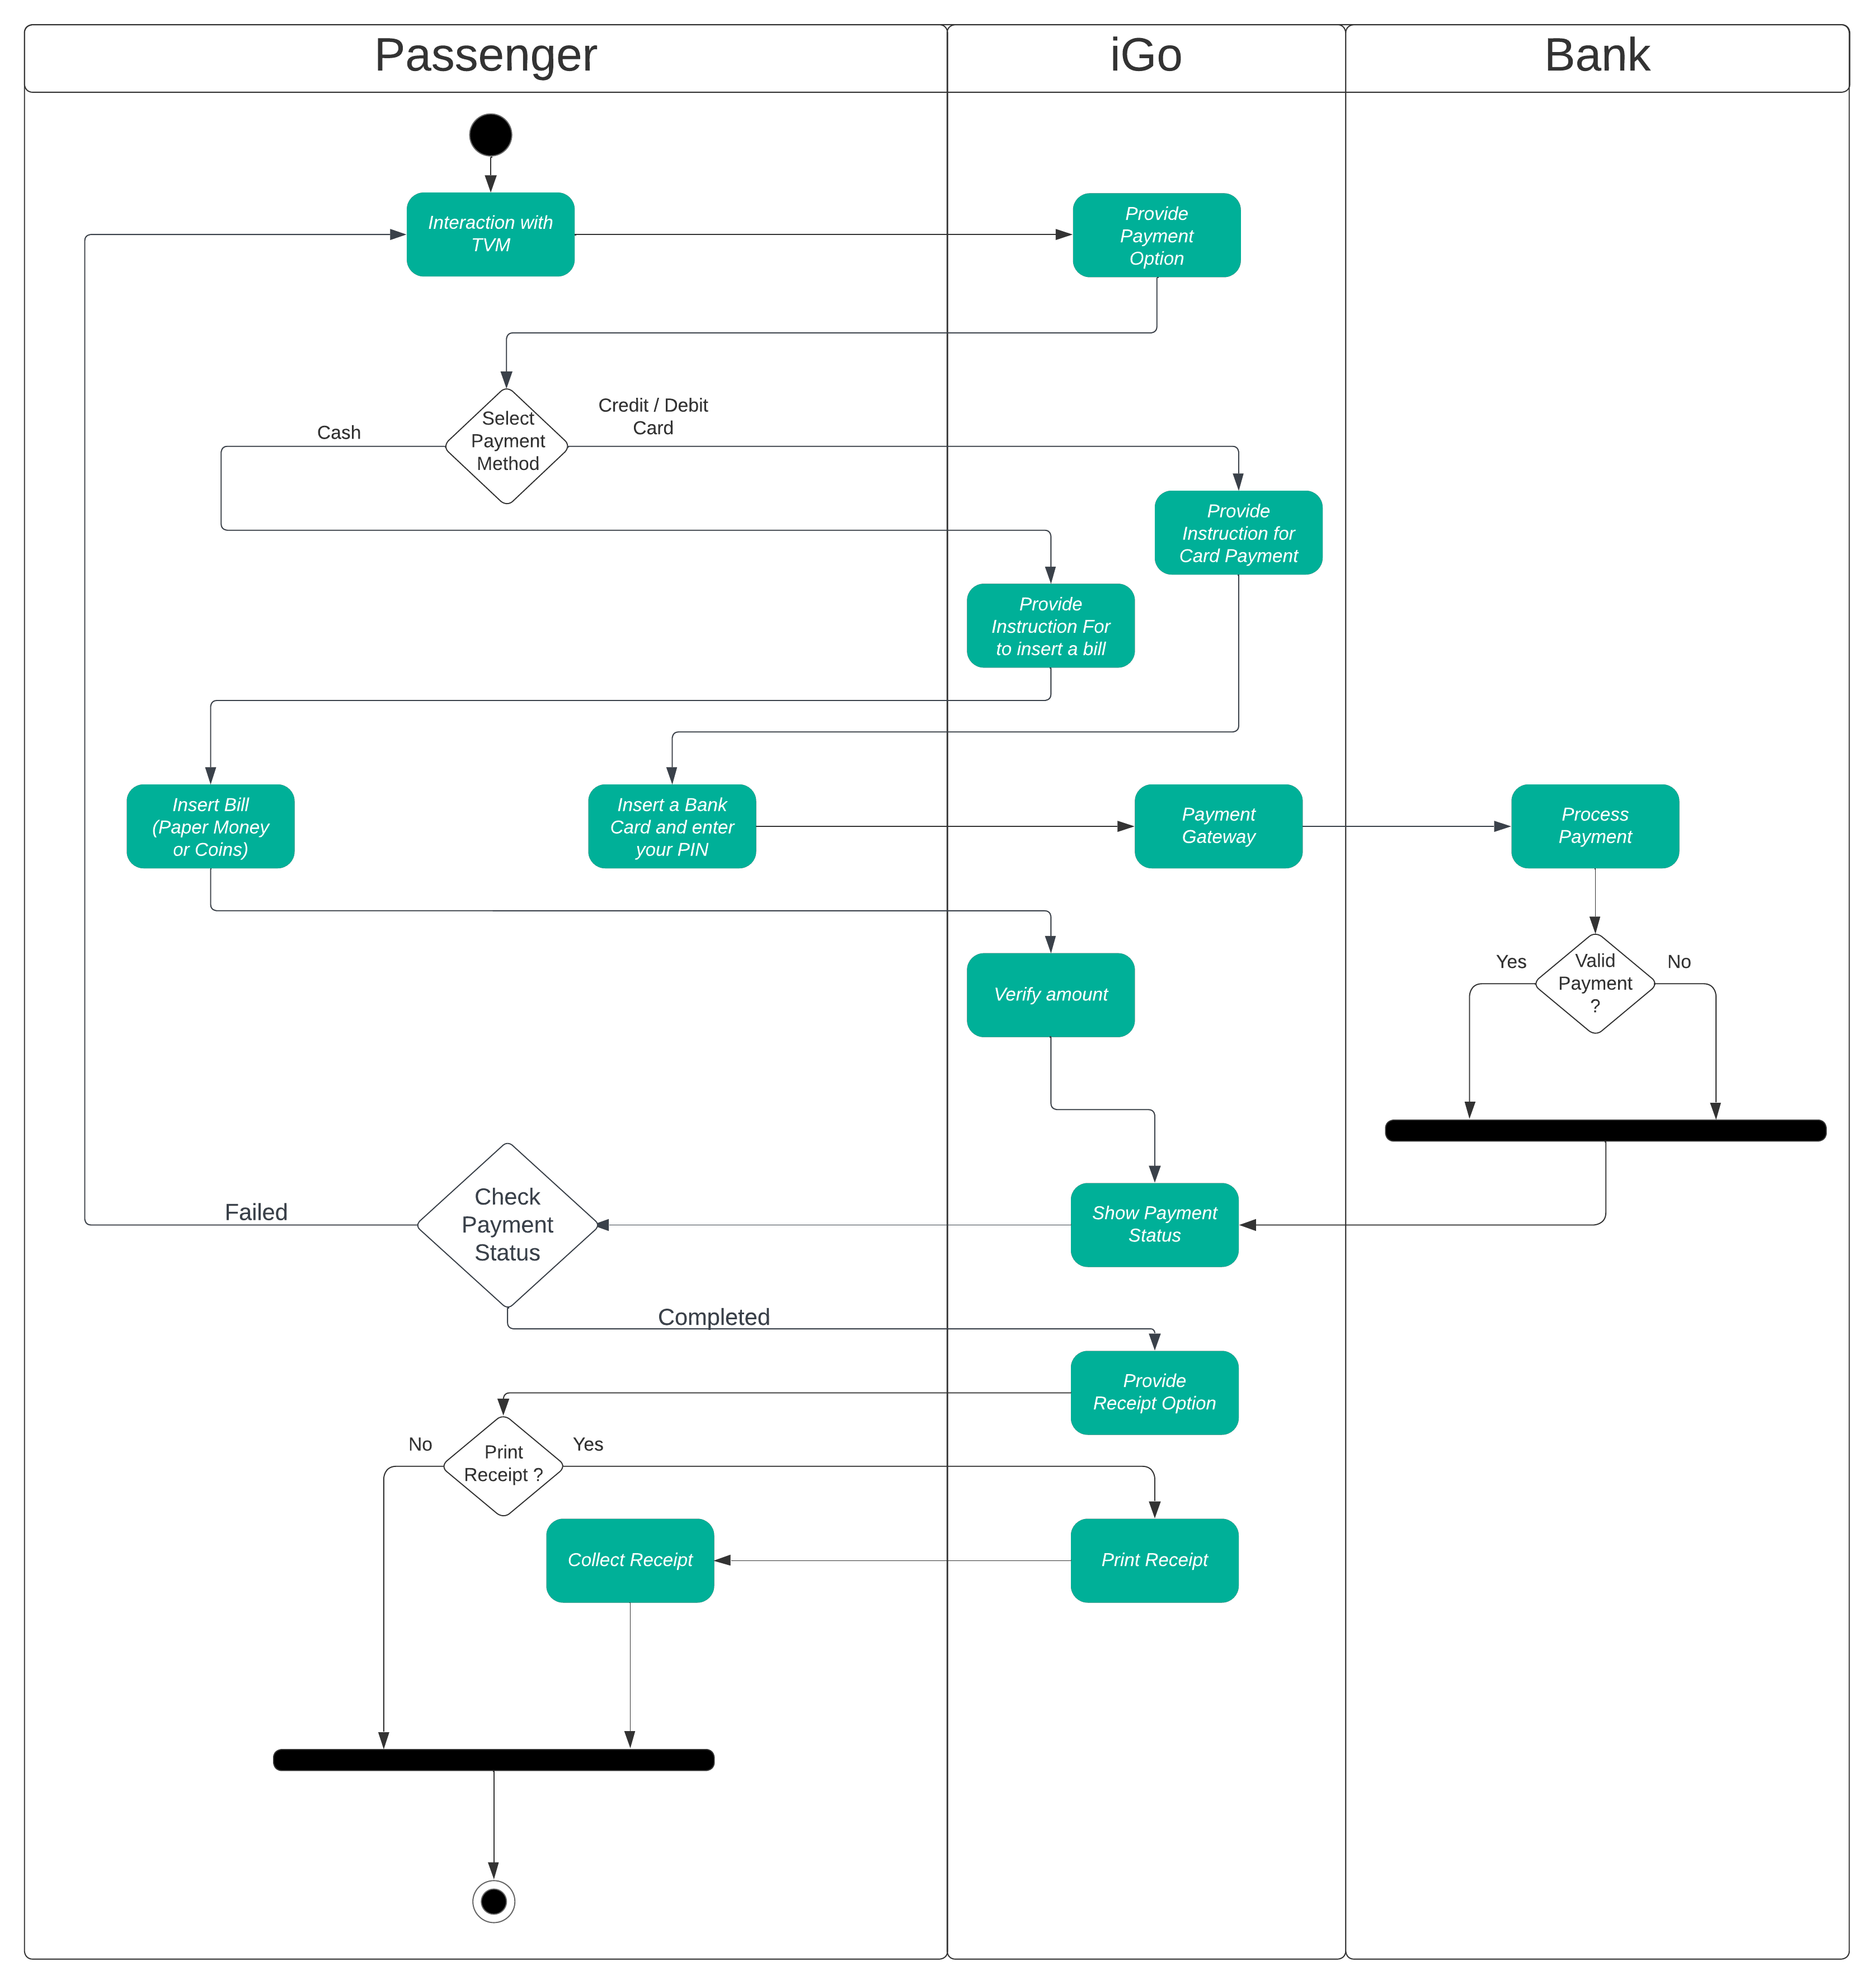
\includegraphics[scale=0.15]{Activity_Diagram_Payment_Method.png}
    \caption{UML Activity Diagram : Payment Method\\ 
    The use case scenario for two payment methods—cash and credit/debit card—is shown in this activity diagram. Following the selection of the selected choice, the system displays the appropriate payment instructions before passing control to the payment gateway to verify the payment, if made with a debit or credit card, or to authenticate it if made with cash. After showing the payment status, a prompt to print a receipt is displayed to the user.}
    \label{fig:Activity Diagram Payment Method}
\end{figure}

\begin{figure}[h]
    \centering
    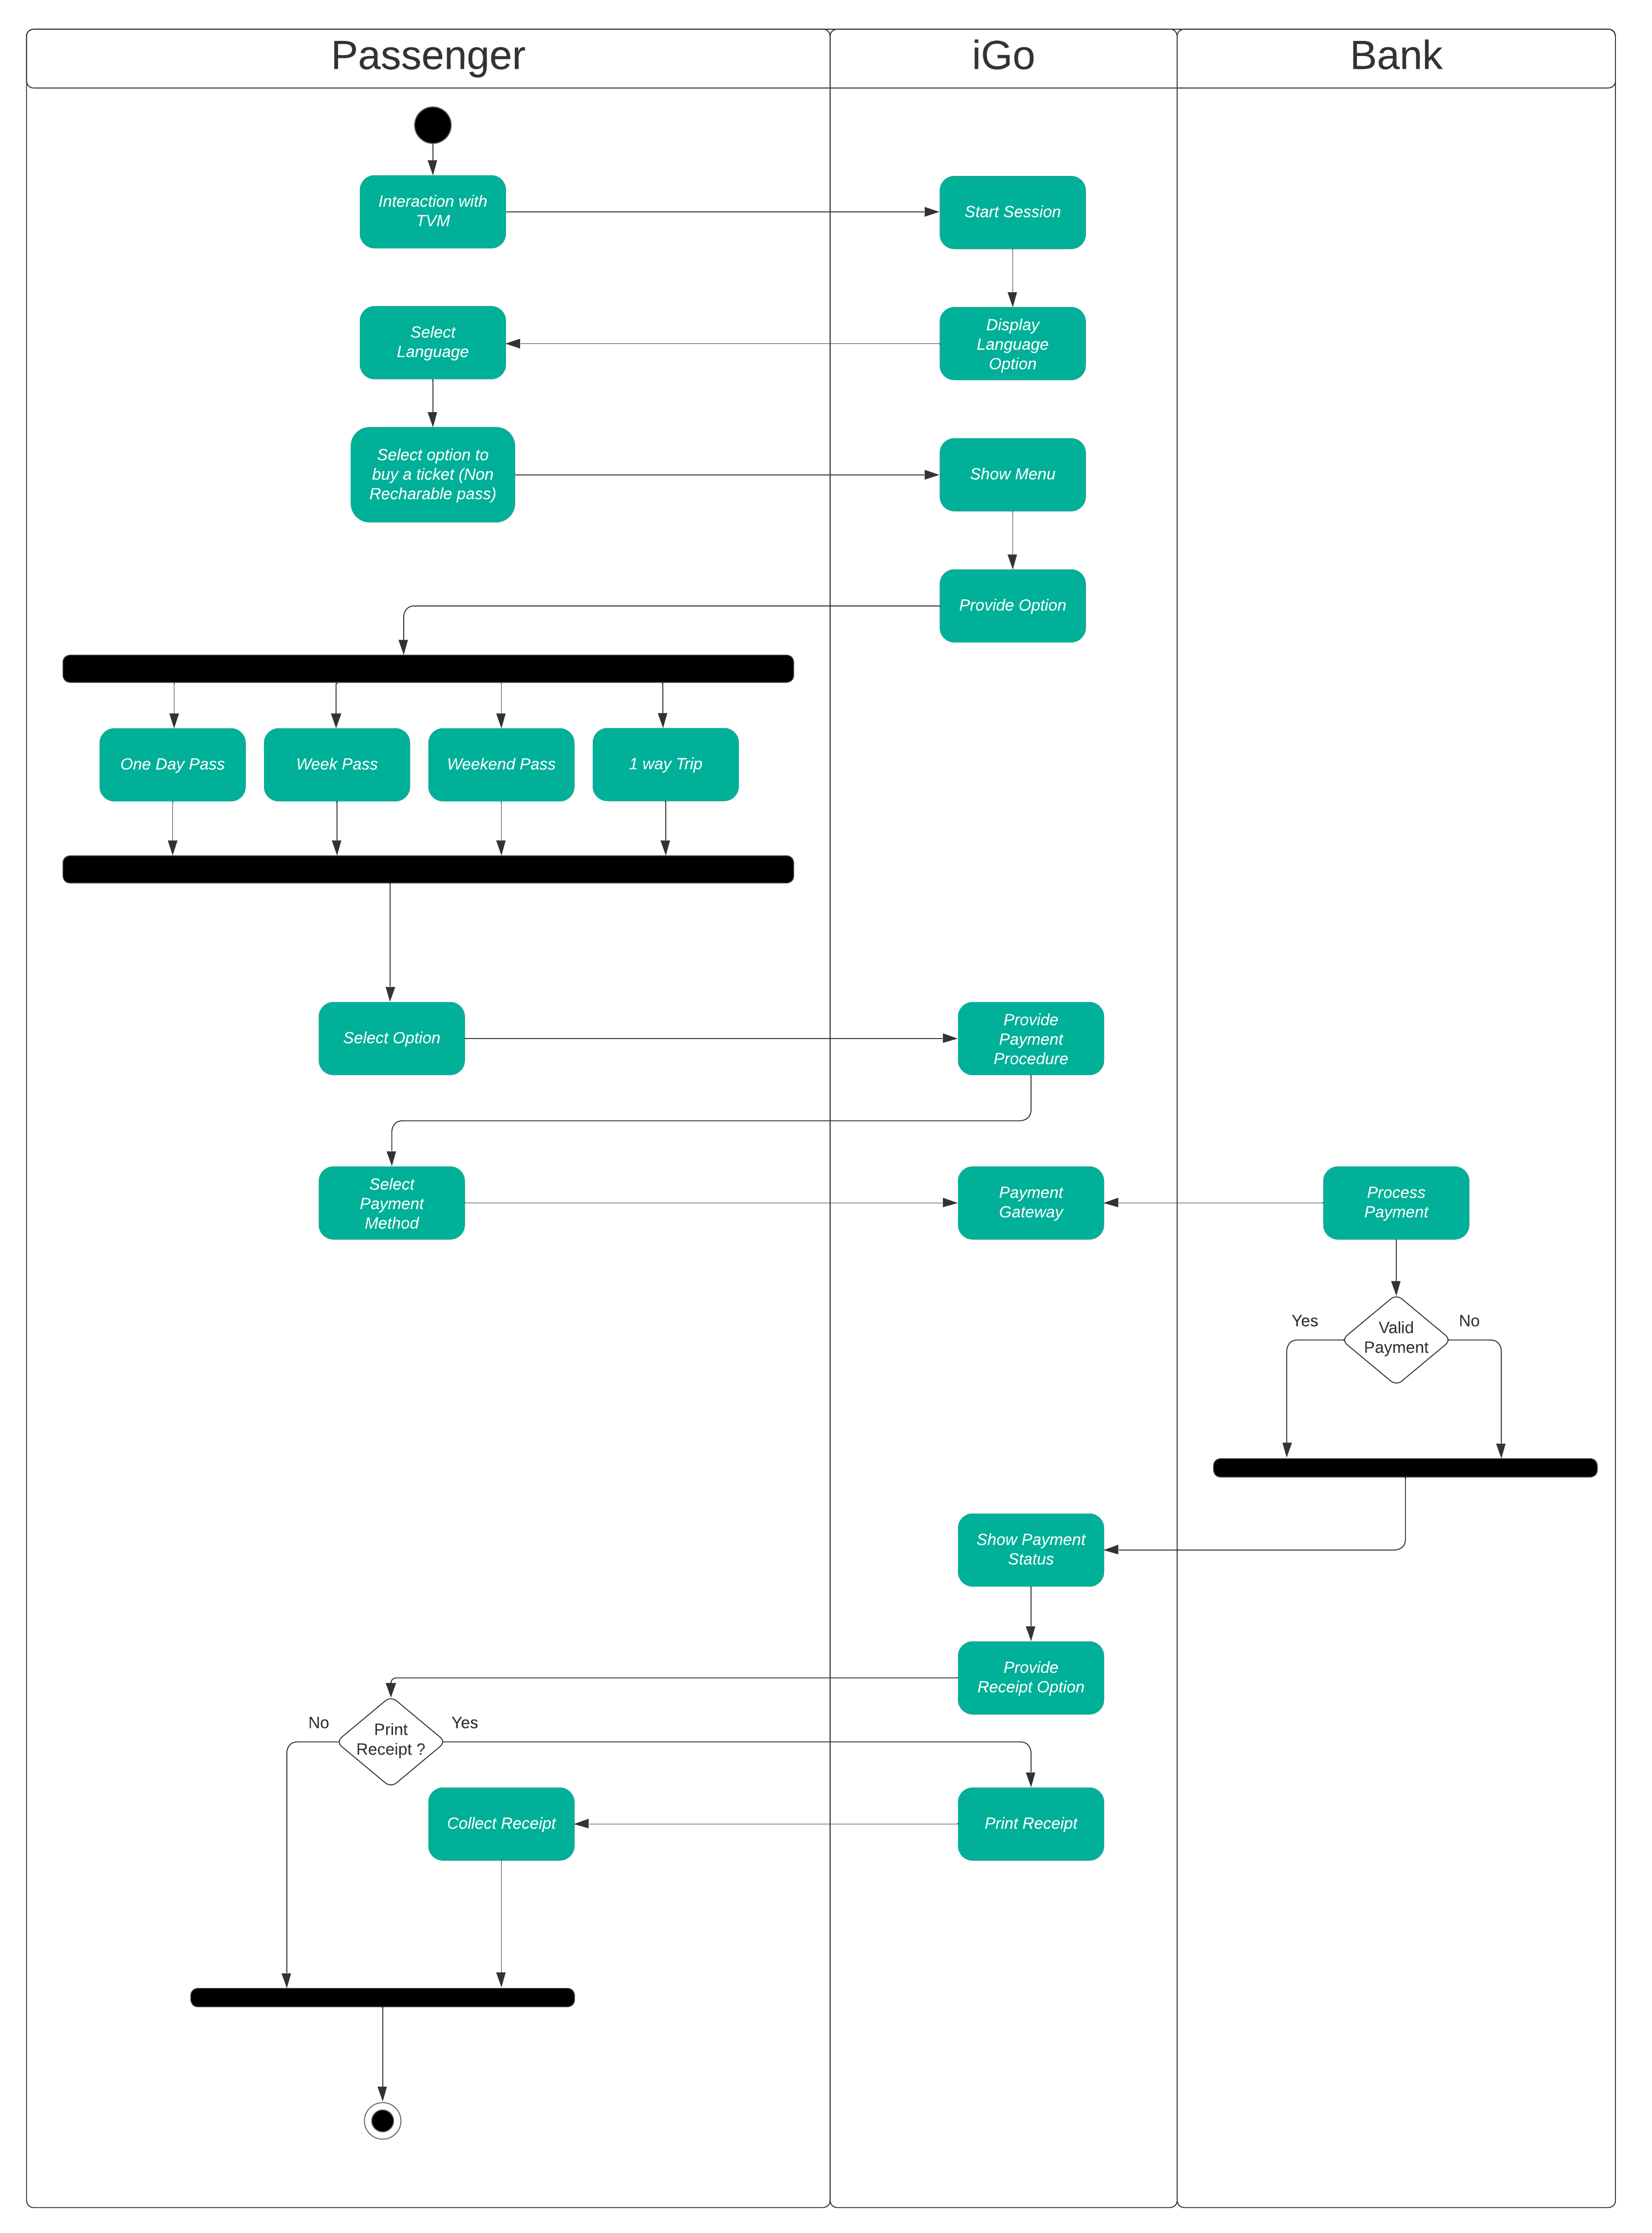
\includegraphics[scale=0.15]{Activity_diagram_Ticket_Purchasing.png}    
    \caption{UML Activity Diagram : Ticket Purchasing \\
    The use case scenario of buying a ticket is illustrated in this activity diagram. It begins by asking the user to choose the option to purchase a ticket, after which a menu is displayed. After choosing an option, the user is then prompted to print a receipt before the control moves to the payment gateway and the payment process is authenticated.\\
    }
    \label{fig:Activity Diagram Ticket Purchasing}
\end{figure} 

\begin{figure}[h]
    \centering
    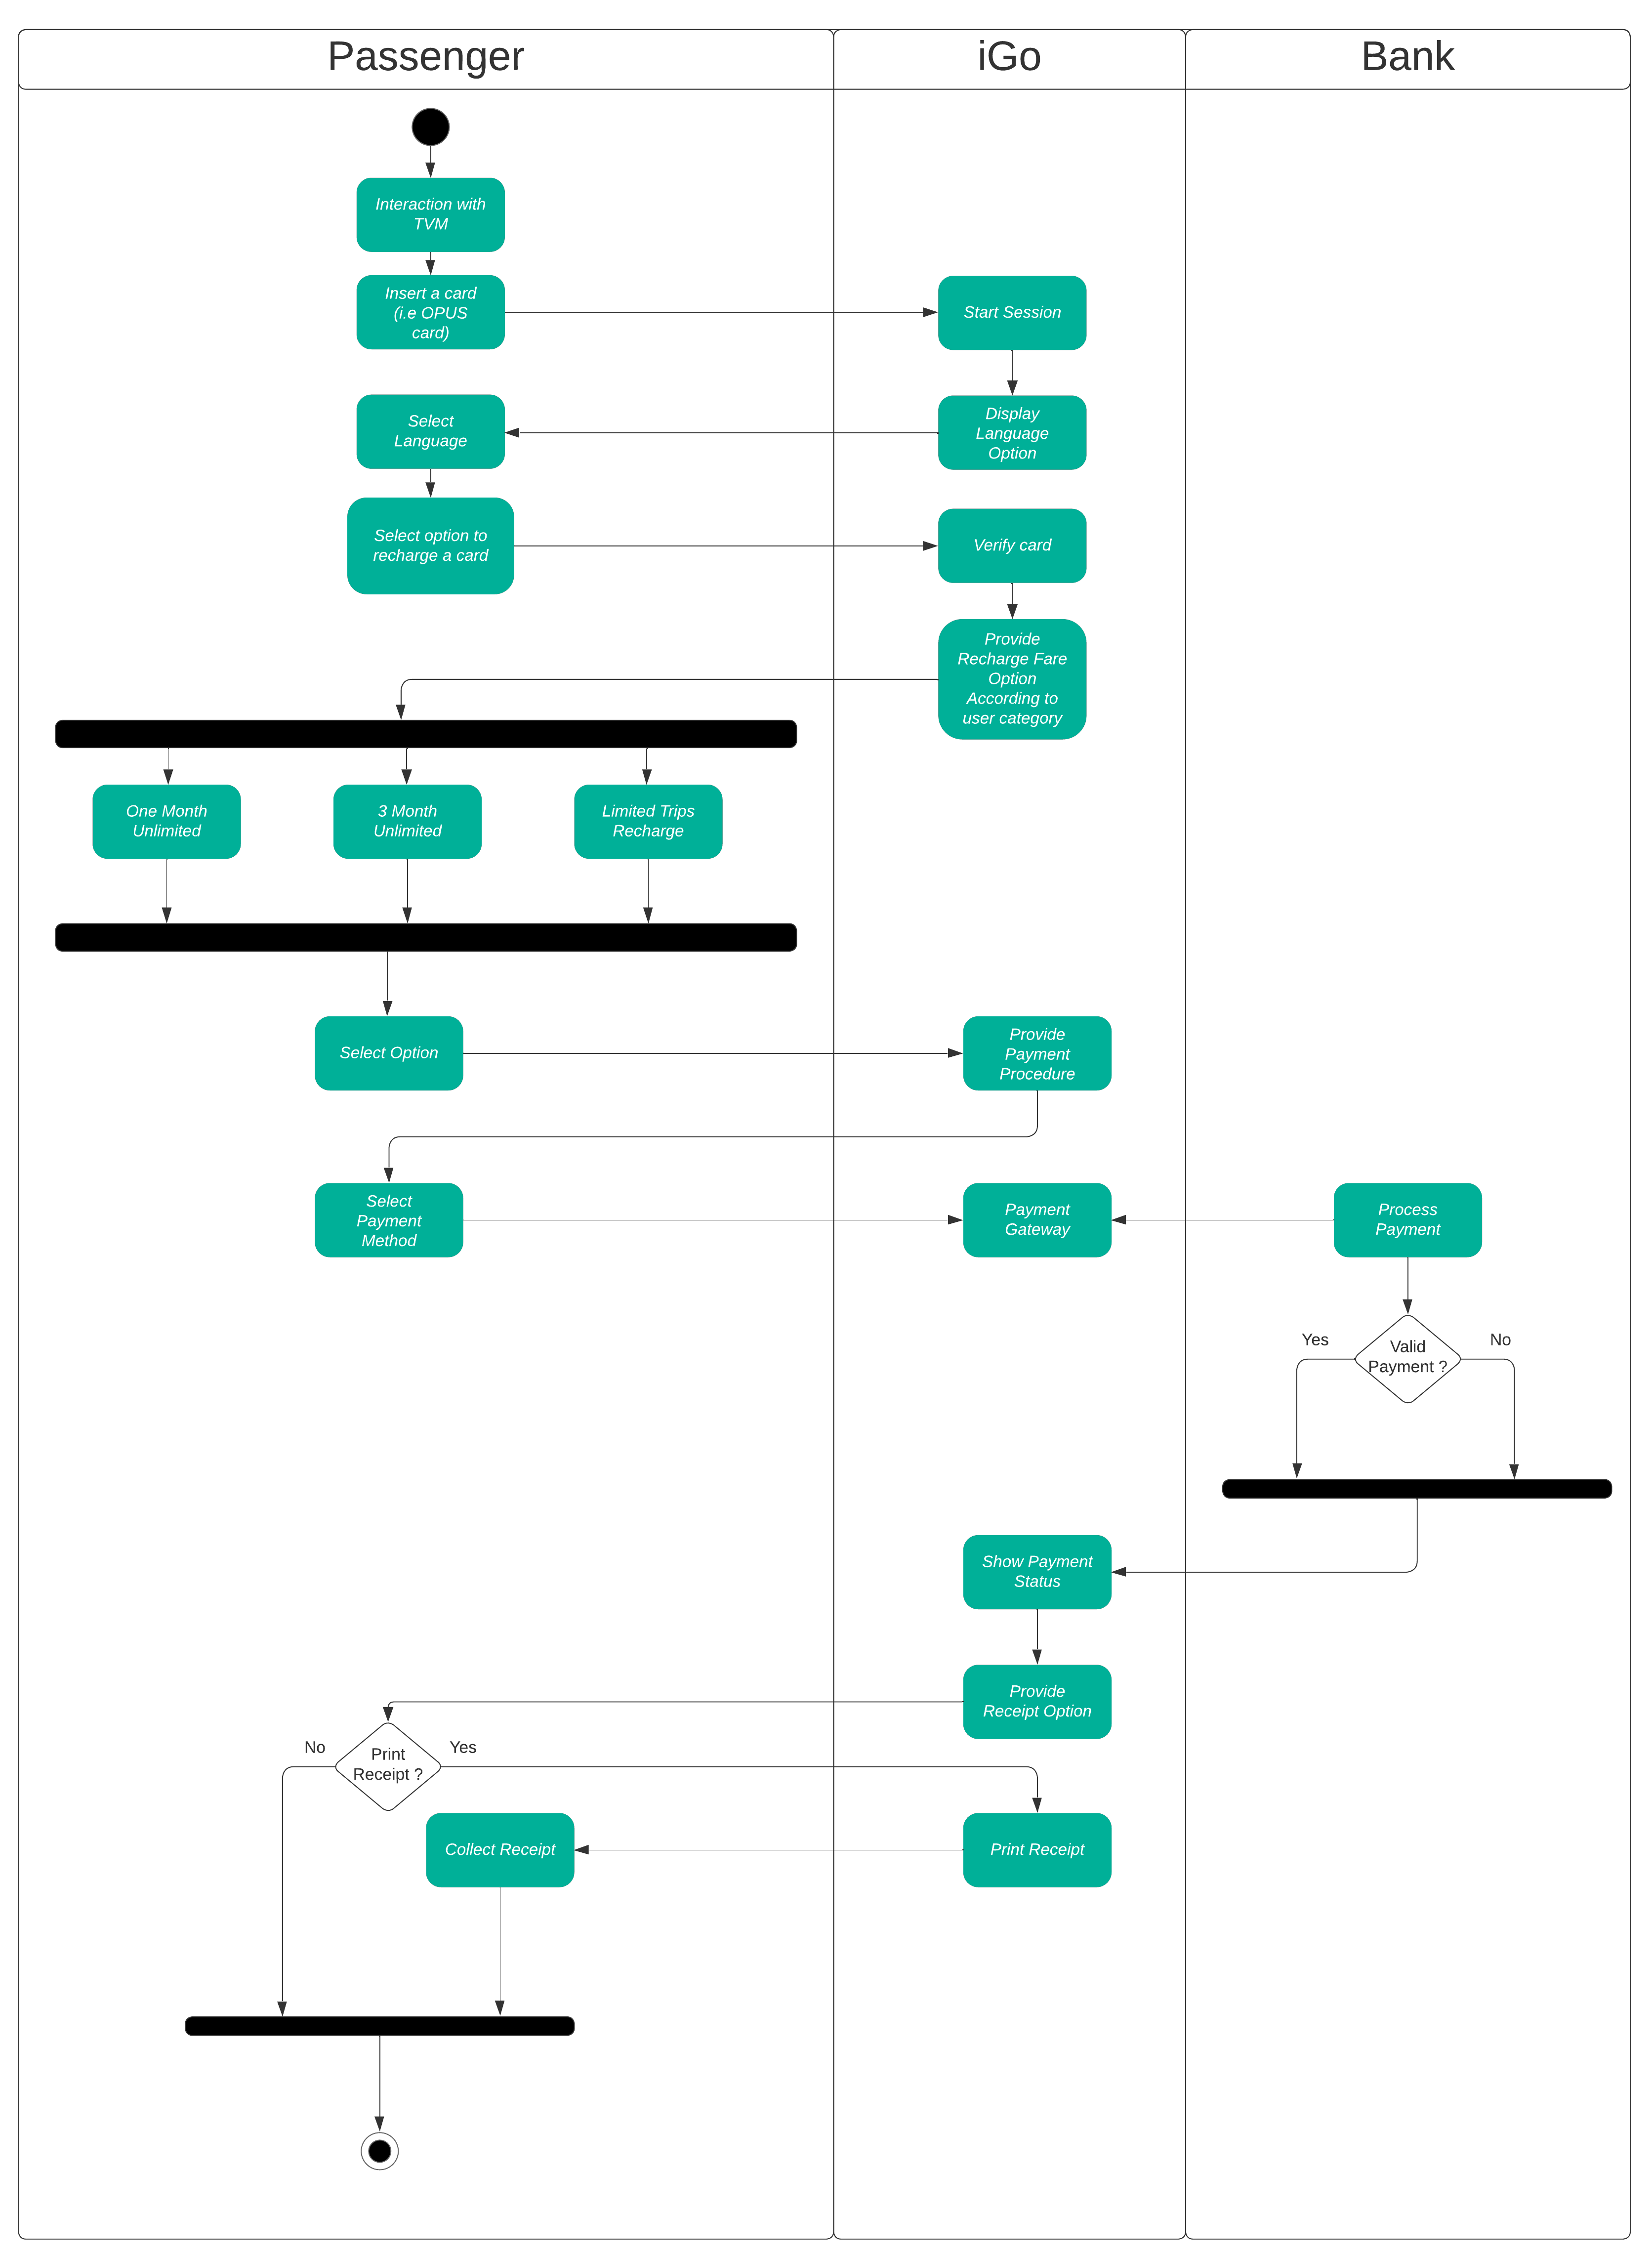
\includegraphics[scale=0.15]{Activity_diagram_Recharge_a_Card.png}
    \caption{UML Activity Diagram : Recharge a Card \\This activity diagram illustrates the use case scenario of recharge an accsess card. It begins by requesting the user to enter their access card, then presents them with a variety of menu alternatives. When the payment is authenticated by the payment gateway, the user is prompted to print the receipt.\\
    }
    \label{fig:Activity Diagram Recharge a card}
\end{figure} 
\begin{figure}[h]
    \centering
    \includegraphics[scale=0.13]{Activity_Diagram_View_Transaction_History.png}
    \caption{UML Activity Diagram : View Transaction History\\ 
    This activity diagram shows the use case scenario for transaction history viewing. If the user chooses the option for transaction history after the options are displayed, a request for information is sent to a remote server. The requested information is displayed if the user chooses Payment Details.}
    \label{fig:Activity Diagram View Transaction History}
\end{figure}
 
\chapter{Glossary}
 \begin{itemize}
\item iGo - iGo	The online Ticket Vending Machine Web Application.
\item Positive Stakeholder- Stakeholder who wishes to make a constructive contribution to the project.
\item Negative Stakeholder- Stakeholder who intends to hurt the project or make a negative contribution.
\item OPUS - The STM travelling card known as OPUS, which is produced and distributed by STM agencies, is used by passengers to travel by the STM metro.
\item TVM - Ticket Vending Machine
\item STM - Société de transport de Montréal public transportation company.
\end{itemize}
\chapter{Tools Used}
 \begin{itemize}
     \item Overleaf
     \item Xmind
     \item LucidChart
     \item GitHub
     \item Google drive
 \end{itemize}
\chapter{References}
\begin{enumerate}
  \item PANKAJ KAMTHAN (2023) “Brainstorming and Mind mapping "
  \item PANKAJ KAMTHAN (2023) “Introduction to Diagramming"
  \item PANKAJ KAMTHAN (2023) “Introduction to Interviews”
  \item PANKAJ KAMTHAN (2023) “Introduction To Domain Modeling”
  \item PANKAJ KAMTHAN (2023) “Introduction To Use Case Modeling” 
  \item \url{https://www.lucidchart.com/pages/uml-activity-diagram}
  \item \url{http://www.stm.info/en}
\end{enumerate}

\chapter{Appendix}
\textbf{\LARGE{Interview Questions}}\\
Interview 1 \href{https://drive.google.com/file/d/14KPH2_q0eTWy8PQVPhdm8psBC041HXt7/view?usp=share_link}{link} \\
Date – 28th February,2023, 5:45 PM\\
Interviewers – Mahavir, Krishna\\
Interviewee – Sharad Patel\\
Q1. - Have you ever used the TVM before? (Yes or no) \\
Ans – Yes\\
Q2. – Have you ever used any public transportation? If yes, how often do you use public transportation? \\
Ans – Yes, Everyday\\
Q3. – Which kind of public transportation you have used the most? (Metro, Bus, or Both)  \\
Ans – Both\\
Q4. – Have you used any TVM at public transportation? (Yes or no) \\
Ans – Yes\\
Q5. – Did you faced any difficulties using the any TVM? (Yes or no) \\
Ans – Yes\\
Q6. – What kinds of difficulties you have faced when using the TVM for the first time? \\
Ans – System Error and if they make any changes in plans or something, like recently they divided Montreal in three zones and they have changed their monthly or weekly plans for different zones. \\
Q7. – How difficult is to use TVM on a scale 1 to 10 for the first time? \\
Ans – 4\\
Q8. – Did you need any guidance when you first encountered the TVM at public transportation? if yes what kind of feasible solution helps to mitigate these problems? \\
Ans – no\\
Q9. – Where do you find the TVM at public transportation? like for at bus station or metro station. \\
Ans – Metro station\\
Q10. – which place do you think is more accessible for the TVM? (Inside the station or outside the station) and why? \\
Ans – Inside the station because of long que and weather outside the station\\
Q11. – have you ever found any differently abled person to use the TVM? (Yes or no) \\
Ans – yes\\
Q12. – How difficult is to use current TVM for the differently abled person on a scale 1 to 10? \\
Ans – 8\\
Q13. – what kind of feasible solution do you think helps to ease the process at TVM for differently abled people? \\
Ans – Long que and waiting time. \\
Q14. – How many TVMs do you usually finds at any station? \\
Ans – One \\
Q15. – do you find any scenario where the TVM was not working at any station? \\
Ans – Yes, many times\\
Q16 – how many TVMs do you think are required for any metro station? and why? \\
Ans – At least five because of long waiting time\\
Q17. – what do you prefer from rechargeable card or non-rechargeable ticket or pass? \\
Ans – Rechargeable card\\
Q18. – does the current TVM support both types of passes like rechargeable card or non-rechargeable card? \\
Ans – yes\\
Q19. – What is the process to get the rechargeable card? \\
Ans – Go to the transport office and they will provide one after identity verification. \\
Q20. -  Do you want to add functionality to the current TVM like to get the rechargeable card from the TVM itself? (Yes or no) \\
Ans – yes\\
Q21. – what kinds of passes or non-rechargeable tickets do you mostly purchase? (Daily, Weekly, 1 day, 3-day, Unlimited evening) \\
Ans – monthly\\
Q22. – which kind of interface do you prefer? (Digital or physical (Mechanical) interface) \\
Ans – digital\\
Q23. – when you have to recharge a card? and usually what kind of fare-option do you select when you are recharging your card? (Monthly, 3-monthly, etc) \\
Ans – monthly\\
Q24. – which type of payment do use the most? (Cash or Card) \\
Ans – card\\
Q25. – which kind of payment receipt do you prefer the most? (Paper-receipt or e-receipt) \\
Ans – e-receipt\\
Q26. – what additional payment option (like apple-pay) do you think can be added to current metro station? and why? \\
Ans – Apply pay and google pay. \\
Q27. – do you think instead of buying the rechargeable card like OPUS is more convenient rather than to use a digital card like you have in your digital wallet in the smart-phone? \\
Ans – Digital wallet card\\
Q28. – which kind pf the payment process do you think is more convenient for you? (Manually or automatic)? \\
Ans – manually\\
Q29. – do you want to add the pre-authorised recharge payment option to your OPUS card? \\
Ans – no\\
Q30. – Do have any other suggestion which you would like to have at the current TVMs at the metro stations? \\
Ans – Digital wallet card and apple pay. \\
\\
Interview 2 \href{https://drive.google.com/file/d/1Hu0Sbab3ANekuTN5JrRPoGAeLahY8LPv/view?usp=share_link}{link} \\
Date – 26th February,2023, 3:41 PM\\
Interviewers – Mahavir, Krishna\\
Interviewee – Kartik Faldu\\
Q1. - Have you ever used the TVM before? (Yes or no) \\
Ans – Yes\\
Q2. – Have you ever used any public transportation? if yes, how often do you use public transportation? \\
Ans – Yes, Everyday\\
Q3. – Which kind of public transportation you have used the most? (Metro, Bus, or Both)  \\
Ans – Both\\
Q4. – Have you used any TVM at public transportation? (Yes or no) \\
Ans – Yes \\
Q5. – Did you faced any difficulties using the any TVM? (Yes or no) \\
Ans – Yes, Sometimes\\
Q6. – What kinds of difficulties you have faced when using the TVM for the first time? \\
Ans – After providing money sometimes ticket doesn’t come out.  \\
Q7. – How difficult is to use TVM on a scale 1 to 10 for the first time? \\
Ans – 7\\
Q8. – Did you need any guidance when you first encountered the TVM at public transportation? if yes what kind of feasible solution helps to mitigate these problems? \\
Ans – no\\
Q9. – Where do you find the TVM at public transportation? like for at bus station or metro station. \\
Ans – Metro station\\
Q10. – which place do you think is more accessible for the TVM? (Inside the station or outside the station) and why? \\
Ans – Inside the station because of harsh weather in Canada\\
Q11. – have you ever found any differently abled person to use the TVM? (Yes or no) \\
Ans – No\\
Q12. – How difficult is to use current TVM for the differently abled person on a scale 1 to 10? \\
Ans – 8\\
Q13. – what kinds of feasible solution do you think helps to ease the process at TVM for differently abled people? \\
Ans – For blind people they can provide plates for direction of use. \\
Q14. – How many TVMs do you usually finds at any station? \\
Ans – Two \\
Q15. – do you find any scenario where the TVM was not working at any station? \\
Ans – No\\
Q16 – how many TVMs do you think are required for any metro station? and why? \\
Ans – Two is enough because of the availability of staff at the service desk. \\
Q17. – what do you prefer from rechargeable card or non-rechargeable ticket or pass? \\
Ans – Rechargeable card\\
Q18. – does the current TVM support both types of passes like rechargeable card or non-rechargeable card? \\
Ans – yes\\
Q19. – What is the process to get the rechargeable card? \\
Ans – visit the STM centre and pay deposit they will provide card after identity verification. \\
Q20. -  Do you want to add functionality to the current TVM like to get the rechargeable card from the TVM itself? (Yes or no) \\
Ans – yes\\
Q21. – what kinds of passes or non-rechargeable tickets do you mostly purchase? (Daily, Weekly, 1 day, 3-day, Unlimited evening) \\
Ans – unlimited evening\\
Q22. – which kind of interface do you prefer? (Digital or physical (Mechanical) interface) \\
Ans – both\\
Q23. – when you have to recharge a card? and usually what kind of fare-option do you select when you are recharging your card? (Monthly, 3-monthly, etc) \\
Ans – monthly\\
Q24. – which type of payment do use the most? (Cash or Card) \\
Ans – card\\
Q25. – which kind of payment receipt do you prefer the most? (Paper-receipt or e-receipt) \\
Ans – e-receipt\\
Q26. – what additional payment option (like apple-pay) do you think can be added to current metro station? and why? \\
Ans – Apply pay is good but it can be added as an alternative option \\
Q27. – do you think instead of buying the rechargeable card like OPUS is more convenient rather than to use a digital card like you have in your digital wallet in the smart-phone? \\
Ans – both digital wallet card and physical card\\
Q28. – which kind pf the payment process do you think is more convenient for you? (Manually or automatic)? \\
Ans – Automatic\\
Q29. – do you want to add the pre-authorised recharge payment option to your OPUS card? \\
Ans – yes\\
Q30. – Do have any other suggestion which you would like to have at the current TVMs at the metro stations? \\
Ans – No\\
\\
Interview 3 \href{https://drive.google.com/file/d/1PnpT-WOk3Vlpm_ruteeafrvHmelRFpJE/view?usp=share_link}{link} \\
Date – 26th February,2023, 4:21 PM\\
Interviewers – Mahavir, Krishna\\
Interviewee – Neha Deshmukh\\
Q1. - Have you ever used the TVM before? (Yes or no) \\
Ans – Yes\\
Q2. – Have you ever used any public transportation? if yes, how often do you use public transportation? \\
Ans – Yes, 4-5 times a week\\
Q3. – Which kind of public transportation you have used the most? (Metro, Bus, or Both)  \\
Ans – Both\\
Q4. – Have you used any TVM at public transportation? (Yes or no) \\
Ans – Yes \\
Q5. – Did you faced any difficulties using the any TVM? (Yes or no) \\
Ans – No\\
Q6. – What kinds of difficulties you have faced when using the TVM for the first time? \\
Ans – language barrier  \\
Q7. – How difficult is to use TVM on a scale 1 to 10 for the first time? \\
Ans – 6\\
Q8. – Did you need any guidance when you first encountered the TVM at public transportation? if yes what kind of feasible solution helps to mitigate these problems? \\
Ans – Yes\\
Q9. – Where do you find the TVM at public transportation? like for at bus station or metro station. \\
Ans – Metro station\\
Q10. – which place do you think is more accessible for the TVM? (Inside the station or outside the station) and why? \\
Ans – Inside the station because of extreme weather conditions \\
Q11. – have you ever found any differently abled person to use the TVM? (Yes or no) \\
Ans – No\\
Q12. – How difficult is to use current TVM for the differently abled person on a scale 1 to 10? \\
Ans – 8\\
Q13. – what kinds of feasible solution do you think helps to ease the process at TVM for differently abled people? \\
Ans – Staff by the STM. \\
Q14. – How many TVMs do you usually finds at any station? \\
Ans – 2-3 for large station and 1 for small station\\
Q15. – do you find any scenario where the TVM was not working at any station? \\
Ans – No\\
Q16 – how many TVMs do you think are required for any metro station? and why? \\
Ans – 4\\
Q17. – what do you prefer from rechargeable card or non-rechargeable ticket or pass? \\
Ans – Rechargeable card\\
Q18. – does the current TVM support both types of passes like rechargeable card or non-rechargeable card? \\
Ans – yes\\
Q19. – What is the process to get the rechargeable card? \\
Ans – Registered yourself at STM office. \\
Q20. -  Do you want to add functionality to the current TVM like to get the rechargeable card from the TVM itself? (Yes or no) \\
Ans – yes \\
Q21. – what kinds of passes or non-rechargeable tickets do you mostly purchase? (Daily, Weekly, 1 day, 3-day, Unlimited evening) \\
Ans – weekly \\
Q22. – which kind of interface do you prefer? (Digital or physical (Mechanical) interface) \\
Ans – Digital\\
Q23. – when you have to recharge a card? and usually what kind of fare-option do you select when you are recharging your card? (Monthly, 3-monthly, etc) \\
Ans – Monthly\\
Q24. – which type of payment do use the most? (Cash or Card) \\
Ans – Card\\
Q25. – which kind of payment receipt do you prefer the most? (Paper-receipt or e-receipt) \\
Ans – e-receipt\\
Q26. – what additional payment option (like apple-pay) do you think can be added to current metro station? and why? \\
Ans – yes it would be awesome. \\
Q27. – do you think instead of buying the rechargeable card like OPUS is more convenient rather than to use a digital card like you have in your digital wallet in the smart-phone? \\
Ans – digital wallet card would be best. \\
Q28. – which kind pf the payment process do you think is more convenient for you? (Manually or automatic)? \\
Ans – Manually\\
Q29. – do you want to add the pre-authorised recharge payment option to your OPUS card? \\
Ans – yes\\
Q30. – Do have any other suggestion which you would like to have at the current TVMs at the metro stations? \\
Ans – Apple Pay \\
\\
Interview 4 \href{https://drive.google.com/file/d/1s_sGqSsWfNolb5bjUEd6yi47pF3mKqgM/view?usp=share_link}{link} \\
Date – 27th February,2023, 11:38 PM\\
Interviewers – Mahavir, Krishna\\
Interviewee – Vishnu\\
Q1. - Have you ever used the TVM before? (Yes or no) \\
Ans – Yes\\
Q2. – Have you ever used any public transportation? if yes, how often do you use public transportation? \\
Ans – Yes, Often\\
Q3. – Which kind of public transportation you have used the most? (Metro, Bus, or Both) \\ 
Ans – Both\\
Q4. – Have you used any TVM at public transportation? (Yes or no) \\
Ans – Yes \\
Q5. – Did you faced any difficulties using the any TVM? (Yes or no) \\
Ans – Yes, Sometimes\\
Q6. – What kinds of difficulties you have faced when using the TVM for the first time? \\
Ans – understanding the buttons. \\
Q7. – How difficult is to use TVM on a scale 1 to 10 for the first time? \\
Ans – 2\\
Q8. – Did you need any guidance when you first encountered the TVM at public transportation? if yes what kind of feasible solution helps to mitigate these problems? \\
Ans – Yes, need a staff near the machine\\
Q9. – Where do you find the TVM at public transportation? like for at bus station or metro station. \\
Ans – Metro station\\
Q10. – which place do you think is more accessible for the TVM? (Inside the station or outside the station) and why? \\
Ans – Inside the station \\
Q11. – have you ever found any differently abled person to use the TVM? (Yes or no) \\
Ans – No\\
Q12. – How difficult is to use current TVM for the differently abled person on a scale 1 to 10? \\
Ans – 7\\
Q13. – what kinds of feasible solution do you think helps to ease the process at TVM for differently abled people? \\
Ans – height of the TVM machine  \\
Q14. – How many TVMs do you usually finds at any station? \\
Ans – Two \\
Q15. – do you find any scenario where the TVM was not working at any station? \\
Ans – No\\
Q16 – how many TVMs do you think are required for any metro station? and why? \\
Ans – 3\\
Q17. – what do you prefer from rechargeable card or non-rechargeable ticket or pass? \\
Ans – Rechargeable card\\
Q18. – does the current TVM support both types of passes like rechargeable card or non-rechargeable card? \\
Ans – yes\\
Q19. – What is the process to get the rechargeable card? \\
Ans – Nearest STM office. \\
Q20. -  Do you want to add functionality to the current TVM like to get the rechargeable card from the TVM itself? (Yes or no) \\
Ans – yes\\
Q21. – what kinds of passes or non-rechargeable tickets do you mostly purchase? (Daily, Weekly, 1 day, 3-day, Unlimited evening) \\
Ans – depends on occasion. \\
Q22. – which kind of interface do you prefer? (Digital or physical (Mechanical) interface) \\
Ans – Digital\\
Q23. – when you have to recharge a card? and usually what kind of fare-option do you select when you are recharging your card? (Monthly, 3-monthly, etc) \\
Ans – monthly\\
Q24. – which type of payment do use the most? (Cash or Card) \\
Ans – card\\
Q25. – which kind of payment receipt do you prefer the most? (Paper-receipt or e-receipt) \\
Ans – e-receipt\\
Q26. – what additional payment option (like apple-pay) do you think can be added to current metro station? and why? \\
Ans – Don’t think that’s required. \\
Q27. – do you think instead of buying the rechargeable card like OPUS is more convenient rather than to use a digital card like you have in your digital wallet in the smart-phone? \\
Ans – digital wallet card would be good. \\
Q28. – which kind pf the payment process do you think is more convenient for you? (Manually or automatic)? \\
Ans – Manually\\
Q29. – do you want to add the pre-authorised recharge payment option to your OPUS card? \\
Ans – yes\\
Q30. – Do have any other suggestion which you would like to have at the current TVMs at the metro stations? \\
Ans – If the put the whole system online rather than the TVM machine\\


\end{document}